\documentclass[../Main.tex]{subfiles} 
\begin{document}

\section{Algorithms}
\subsection{Data structure and overview}
Our basic datastructure is a vector whose dimensions represent regions, thus we use seven-dimensional vectors for working with our seven defined regions.
We apply vectors one the one hand to words (types) and on the other hand to Tweets (documents). They show the strength of the word's or the Tweet's affiliation to the individual regions.

So for instance the Word \textit{Porree} could be equally significant for the regions \textit{Ostdeutschland, Norddeutschland} and \textit{Westdeutschland}. Consequently we would guess the probability that a usage of this word indicates origin from one of these regions to be one third for each of them, and to be zero for each of the other regions.

$$\vec V_{Porree} = \begin{pmatrix} 0,33 \\ 0,33 \\ 0,33 \\ 0,0 \\ 0,0 \\ 0,0 \\ 0,0 \end{pmatrix} \ \ \ \ \begin{matrix} \text{Ostdeutschland} \\ \text{Norddeutschland} \\ \text{Westdeutschland} \\ \text{Bayern} \\ \text{Südwestdeutschland} \\ \text{Schweiz} \\ \text{Österreich} \end{matrix}$$

As a seed we use initial word vectors \textit{(generation 0}. What comes next is an accumulation stage, during which more regionally salient words are supposed to be found using training data from Twitter. This is done by our main algorithm, which calculates a following generation of word vectors from a previous one. Thus it can be executed in a loop running any number of cycles you like. Eventually we get a final generation of word vectors, from which we then calculate the average vector (normalized to length 1). At this stage our model has passed training and is ready to be applied.

In application phase an unseen Tweet comes in. We calculate a Tweet vector for it and subtract it from the average vector. The difference vector shows the region we eventually assign the Tweet to.

\subsection{Main algorithm}
The main algorithm calculates a new generation of word vectors based on an existing generation and a training corpus of Tweets.

It iterates over all Tweets in the corpus. For each Tweet a Tweet vector is calculated. Therefore the existing generation's word vector for each token in the Tweet simply is added, provided it exists. Subsequently, the resulting Tweet vector conversely is added to the new generation's word vector. In case any of the Tweet's tokens are not represented in the old generation of word vectors they now join for the new generation; thus the number of word vectors increases. Values for already existing words do also change, though.

In a nutshell, first a Tweet vector is calculated for each Tweet in the training corpus based on the existing generation's word vectors for the Tweet's words, and then a word vector is calculated for each word in the corpus based on the Tweet vectors for all the Tweets the word occurs in.\\

\begin{algorithm}[H]
 \SetAlgoLined\DontPrintSemicolon
 \KwData{\\
  $WV_0$: existing set of word vectors $WV_0(word) = \vec V_{word}$\\ 
  $Tweets$: set of Tweets\\
  \vspace{1em}
 }
 \KwResult{\\
  $WV_1$: enriched set of word vectors $WV_1(word) = \vec V_{word}$\\
  \vspace{1em}
 }
 $WV_1 \gets\emptyset $\;
 \ForEach{Tweet in Tweets}{
  $\vec V_{Tweet} \gets (0,0,0,0,0,0,0)$\;
  \ForEach{Token in Tweet}{
   $\vec V_{Tweet} \gets \vec V_{Tweet} + WV_0(Token)$\;
  }
  \ForEach{Token in Tweet}{
   $WV_1(Token) \gets WV_1(Token) + \vec V_{Tweet}$\;
  }
 }
 \ForEach{$\vec V_{Word}$ in $WV_1$}{
  $\vec V_{Word} \gets \text{normalize}(\vec V_{Word})$\;
 }
 \Return $WV_1$\;
 \caption{Tweegion main algorithm}
\end{algorithm}

\subsection{Difference between both attempts}
The difference between the regional word attempt and the geo location attempt lies in the seed for the main algorithm. For the regional word attempt we manually defined about 200 initial word vectors based on a source for regional expressions.

With the geo location attempt, by contrast, we have the initial word vectors learned by machine, too. For this purpose we use a special collection of geo annotated Tweets. Based on its coordinates each Tweet is assigned to one of our seven regions. Similarly as we do it in the main algorithm, we now calculate word vectors based on the Tweets the words occur in.

Our results are ten thousands of initial word vectors for the geo location attempt depending on the size of the special training corpus. So this attempt tendentially needs less cycles of the main algorithm for the same amount of final word vectors.

\subsection{Normalizing versions}
Over the course of our work we developed multiple versions of our main algorithm which differ in treatment of the word vectors at the end of each cycle, i. e. subsequent to the calculation of Tweet and word vectors. This treatment directly affects the following calculation of Tweet vectors, be it in a possible further cycle of the main algorithm or in the application stage, i. e. for classifying an unseen Tweet.

The original version, \textit{Normalized,} includes a normalization of all word vectors to sum 1. This means every type is equivalent regardless of the number of tokens. During test runs we found this approach to have an extreme bias towards rare words, since they only occur in one or a few Tweets and are therefore graded strongly salient for a certain region.

$$\text{normalize}(\vec v) = \frac{\vec v}{\sum_i v_i}$$

Our second version, \textit{Linear,} then came into being by simply omitting the normalization. With this approach, every type now has a weight directly linearly dependent on its frequency as a token. This alternative however, as it turned out, lended high frequent words such a huge weight that regional salience, being more common with words of medium frequency, suffered a heavy loss and only tiny deviations from the average vector remained.

$$\text{normalize}(\vec v) = \vec v$$

Driven by this experiences we decided to find a trade-off between constant and linear dependency. So we developed the version \textit{Log,} where the vector's length is changed in such a way, that its sum increased by 1 thereby is logarithmized to base 2.

$$\text{normalize}(\vec v) = \frac{\vec v}{\sum_i v_i} * \log_2(\sum_i v_i+1)$$

In the case of \textit{Root,} the square root is used rather than the logarithm to base 2.

$$\text{normalize}(\vec v) = \frac{\vec v}{\sum_i v_i} * \sqrt{\sum_i v_i}$$

\subsection{Classifying a tweet}
During application an unseen Tweet is entered and is to be assigned to a region. For this purpose a Tweet vector is calculated for it. This is done by searching its text for words we have got word vectors for. All word vectors we find are then added up.

Afterwards the cosine similarity between the Tweet vector and the average vector is calculated. In case of too large similarity no classification is carried out, see the chapter \textit{Cosine similarity.} 

In the event of the Tweet vector being salient enough it is now normalized to length 1. For assigning the Tweet to one of the regions the difference between the average vector and the Tweet vector is calculated, this giving a difference vector pointing to the direction searched for. More precisely, the vector's maximum value reveales the region the vector points to the most. This region is the result of our classification.

\subsection{Cosine similarity}
\begin{figure}[t]
  \[ sim(\vec{q},\vec{d_j}) = \frac{\sum^N_{i=1} w_{i,q} \times w_{i,j}}{\sqrt{\sum^N_{i=1}w^2_{i,q}} \times \sqrt{\sum^N_{i=1}w^2_{i,j}}} \]
  \caption{Cosine similarity}
  \label{cos_sim}
\end{figure}

\begin{figure}[b]
 \begin{align*}
  q &= \textrm{'Ich glaube @Drahflow tippt noch schneller als er redet. ;) \#om13' } \\
  \vec{q} &= (0.427, 0.38, 0.4, 0.39, 0.391, 0.602,  0.41) \\ 
   \vec{\bar{d}} &= \frac{\sum^N_{i=0} d_i}{N} =  (0.376, 0.336, 0.349, 0.346, 0.361, 0.481,  0.379) \\
  sim(\vec{q}, \vec{\bar{d}}) &= 0.9986 
\end{align*}
  \caption{Example for the similarity calculation}
  \label{cos_sim_example}
\end{figure}
Although Tweets may differ from one region to another in some way, a huge percentage of the German Twitter users write their messages exclusively in standard German with no signs of any regional influence whatsoever. \\
For example the following Tweet just appeared in one of our timelines:
\begin{quote}
'Ich glaube @Drahflow tippt noch schneller als er redet. ;) \#om13'
\end{quote}
Keeping in mind that usernames, hashtags, smileys and punctuation are being removed in the pre-processing, this Tweet contains way too ordinary words to be assigned to a specific region. It is written in pure standard language and therefore could be sent from a village in Bavaria as well as from Berlin, and depending on the data we use to train our algorithm with, the result of the program could be \textit{Österreich} or \textit{Norddeutschland} as well.

\begin{figure}[t]
  \begin{center}
   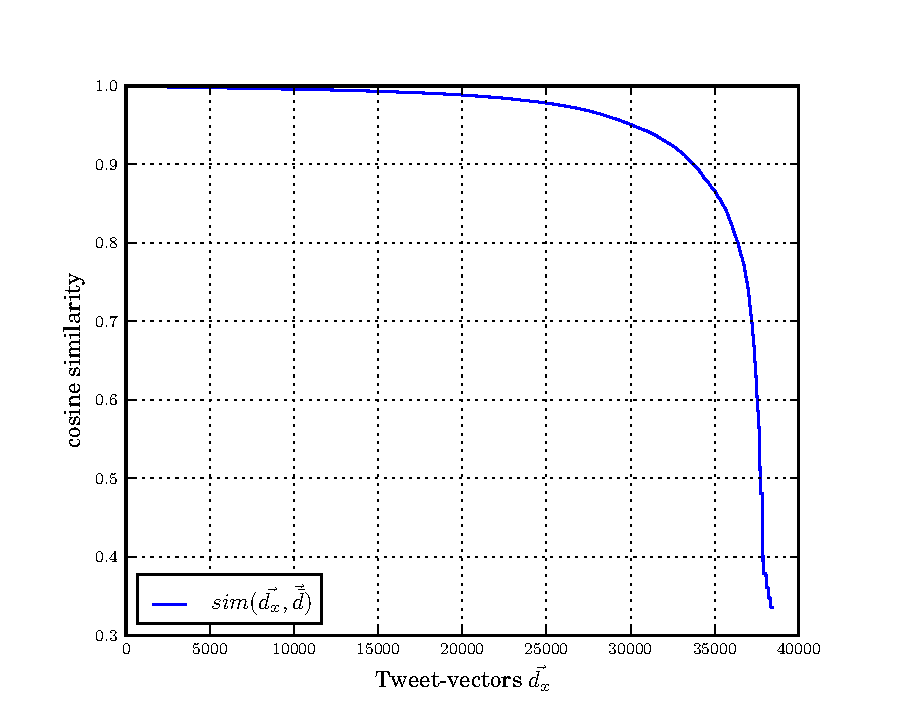
\includegraphics[width=\columnwidth]{../img/cos-verteilung.eps}
    \caption{\label{cos_distribution} Cosine similarity between all Tweet-vectors and the average Tweet-vector}
  \end{center}
\end{figure}

To face this problem we decided to filter this kind of indistinguishable Tweets in order to get more reliable results, thus increasing the accuracy of the algorithm. \\
Our idea was to determine the average Tweet-vector $\vec{\bar{d}}$ of all the Tweets in the training-corpus and to compare the Tweet-vector $\vec{q}$ of an inputted Tweet with it, using the cosine metric (see Figure \ref{cos_sim}) as recommended in \cite[805]{SaLP}. If the similarity between both vectors is smaller than a specified threshold, we continue to map the Tweet to one of the region, otherwise we stop and return a message that the Tweet is written in standard German hence cannot be classified. In the example in figure \ref{cos_sim_example}, the vector $\vec{q}$ for the Tweet mentioned above is compared to the average Tweet-vector $\vec{\bar{d}}$, returning a very high similarity of $0.9986$. Nevertheless the raw algorithm would state the Tweet was most likely sent from Switzerland.

The most difficult part was to find the right threshold that separates the too ordinary Tweets from the significantly regional ones. To make a guess which percentage of all Tweets are written in standard German, we calculated the cosine similarity of all Tweets in the training-corpus to the average vector, sorted them and had a look at the distribution (figure \ref{cos_distribution}). \\
The result was not surprising: More than 80\% of all Tweets had a similarity of 0.9 or higher. Or, seen from another point of view, only 20\% of all Tweets differ enough from the average vector to calculate reliable results.

The result of  the algorithm we created (see algorithm \ref{cos_algorithm)}, is depending on the Tweets to calculate the average vector, a guess of the amount of regional Tweets and the set of word-vectors,  which is created in the main-algorithm. By default, the Tweets are the same dataset as used in the main-algorithm. We decided to use a guess on which the similarity threshold is computed instead of directly entering a value for the threshold. This way, we receive more reliable results and are able to compare the use of different datasets.

In the experiments in the sections \ref{geo_guessing} (geo location based) and 4 (regional based attempt) we tested different thresholds to find a good balance between a reliable classification with a high accuracy and the coverage of as many Tweets as possible.\\

\begin{algorithm}
 \SetAlgoLined
 \KwData{\\
	$tweets$: Set of geo-annotated documents\\ 
	$guess$: $0 \leq guess \leq 1$, guessed amount of regional Tweets\\
	$WV$:  Set of word-vectors}
 \KwResult{\\$threshold$: $0 \leq threshold \leq 1$, cosine similarity threshold}
 $tweetvectors \gets\emptyset $\; 
\ForEach{tweet in tweets}{
$\vec{tweet} \gets (0,0,0,0,0,0,0)$\;
 \ForAll{token in tweet}{
  \If{token $\in$ WV}{
     $\vec{tweet} \gets \vec{tweet} + WV(token)$\;
   }
  $tweetvectors \gets tweetvectors \cup \{\vec{tweet}\}$\;
}
}
$\vec{average} \gets (0,0,0,0,0,0,0)$\;
 \ForEach{$\vec{tweet}$ in $tweetvectors$}{
$\vec{average} \gets \vec{average} + \vec{tweet}$\;
}
$\vec{average} \gets \dfrac{\vec{average}}{l(tweetvectors)}$\;
$vectorlist \gets \emptyset$\;
 \ForEach{$\vec{tweet}$ in $tweetvectors$}{
$similarity \gets sim(\vec{tweet}, \vec{average})$\;
$vectorlist \gets append(similarity)$\;
}
$vectorlist.sort()$\;
$threshold = vectorlist[int(guess \times l(vectorlist))]$\;
\Return $threshold$\;
\caption{Cosine similarity calculation algorithm}
\label{cos_algorithm}
\end{algorithm}

% \subsection{Evaluation}

\end{document}
